The \gls{nfc} describes the plethora steps that nuclear fuel goes through
in its life cycle. In Figure \ref{fig:once-through} we have outlined a
simple "once-through" fuel cycle (so called because the fuel goes through
the cycle once in its lifetime). Nuclear fuel has the capacity to be
reprocessed and recycled into a different fuel type that can produce
usable power for several cycles, called a "closed" fuel cycle.

\begin{figure}[h]
    \centering
    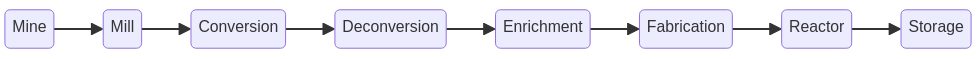
\includegraphics[scale=0.6]{images/once_through_fc.png}
    \caption{US Once-through Fuel Cycle}
    \label{fig:once-through}
\end{figure}

 In the US, we keep each of these facilities separate in the front-end of
 the fuel cycle in a "collect and wait" pathway \cite{cycle_risks}. In
 lieu of a long or interim solution for the \gls{uf}, the back end of the
 \gls{nfc} is collocated with the reactors that burn the fuel (with the
 minor exception of the consolidated storage facility in Morris Illinois).
